
\subsection{Test Project Generation}

Creating a project to test a Qt-based GUI is really easy by using TUG
Wizard. Please, follow the steps described in the following.

%\setcounter{enumi}{4}
\begin{enumerate}
%
%%% Select panel file
%%
\item {\bf Step 1: Select a panel.}\\
%
  Panel is the window to test. \\Click \field{1.1 Select} to select a Qt
  *.ui file.  \field{Class name} will be auto-filled based on the
  panel name found in the selected file. Please, check it.\\
%
  A test project can be also generated without a *.ui file. For this,
  select \field{There is no panel file to test} and fill \field{Class name}
  manually with a name for the panel.\\
%
  Within a Qt GUI, widgets can be referenced in many different ways (e.g.,
  by using a private implementation). By default, widgets are referenced
  using {\tt ui->}. It can be changed selecting \field{Referenced as} and
  filling this field.\\
%
  After this change, a new include could be needed. If so, select
  \field{Add this include} and click \field{1.2 Select} to select a file to
  include.\\
%
  Click \field{Next Step} at the bottom of the wizard.

\vspace{3ex}
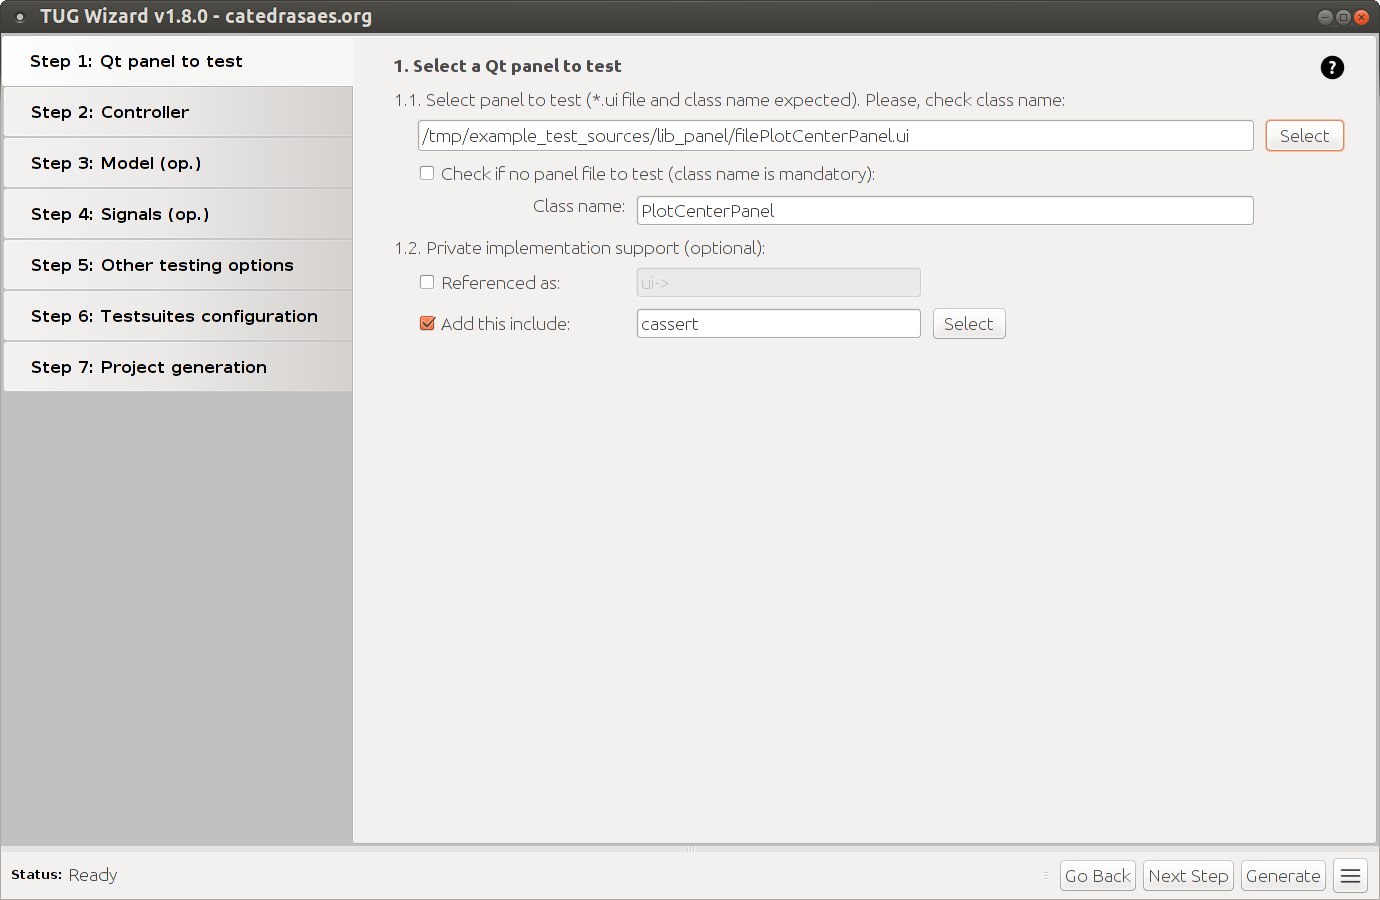
\includegraphics[width=.95\textwidth]{images/tug021.png}
\vspace{3ex}
\newpage
%
%%% 
%%
\item {\bf Step 2: Select Gateway class.}\\
%
  Gateway class (GW) is the class implementing communication with the
  manager (M).\\ 
%
  Click \field{2.1 Select} to choose the library containing the GW
  class. \\
% 
  Click \field{2.2 Select} to select the file defining the GW
  class. \field{Class name} will be auto-filled based on the class name
  found in the selected file. Please, check it. \\
% 
  Click \field{2.3 Select} to select the directory in which GW library is
  built. It is needed if coverage analysis is enabled.\\
%
  In \field{2.4} you can add additional dependencies for the GW
  library. There are some buttons to help you adding dependencies:
  \field{Add dynamic library} and \field{Add includes directory} include
        {\tt qmake} tags; \field{Add file} and \field{Add directory} can be
        used to add new paths. \\
%
  Click \field{Next Step} at the bottom of the wizard.

\vspace{3ex}
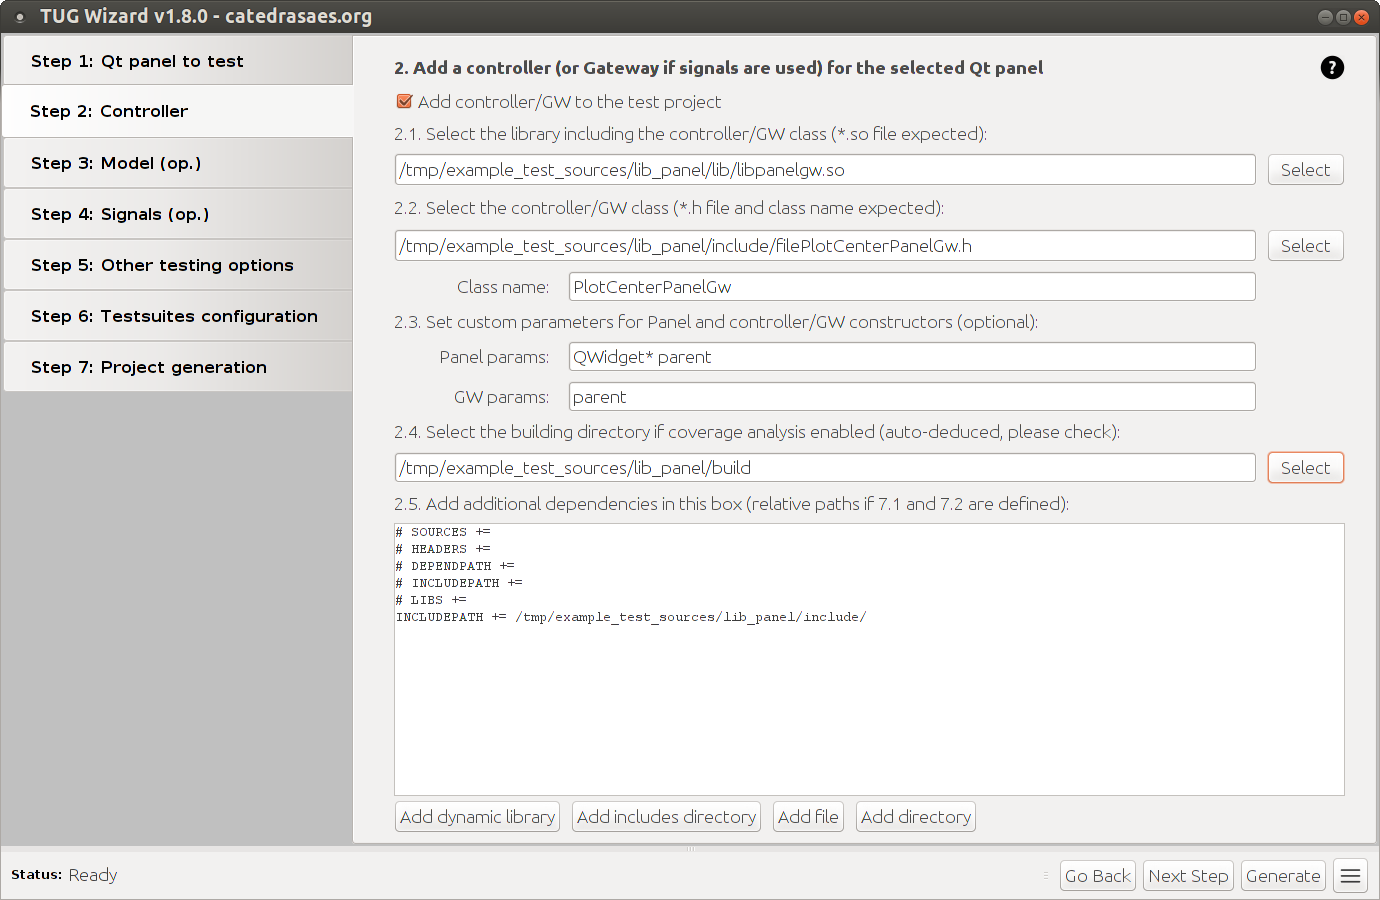
\includegraphics[width=.95\textwidth]{images/tug022.png}
\vspace{3ex}
\newpage
%
%%% 
%%
\item {\bf Step 3: Select a Manager/model (optional).}\\
%
  You can select a manager class (M) with which the panel is connected.\\
%
  Check \field{Include a manager into the testsuites} to enable this
  option. \\
%
  Click \field{3.1 Select} to choose the library containing the M class.\\
%
  Click \field{3.2 Select} to select the file defining the M
  class. \field{Class name} will be auto-filled based on the class name
  found in the selected file. Please, check it.\\
% 
  Click \field{3.3 Select} to select the directory in which M library is
  built. It is needed if coverage analysis is enabled.\\
%
  In \field{3.4} you can add additional dependencies for the M library.\\
%
  Click \field{Next Step} at the bottom of the wizard.

\vspace{3ex}
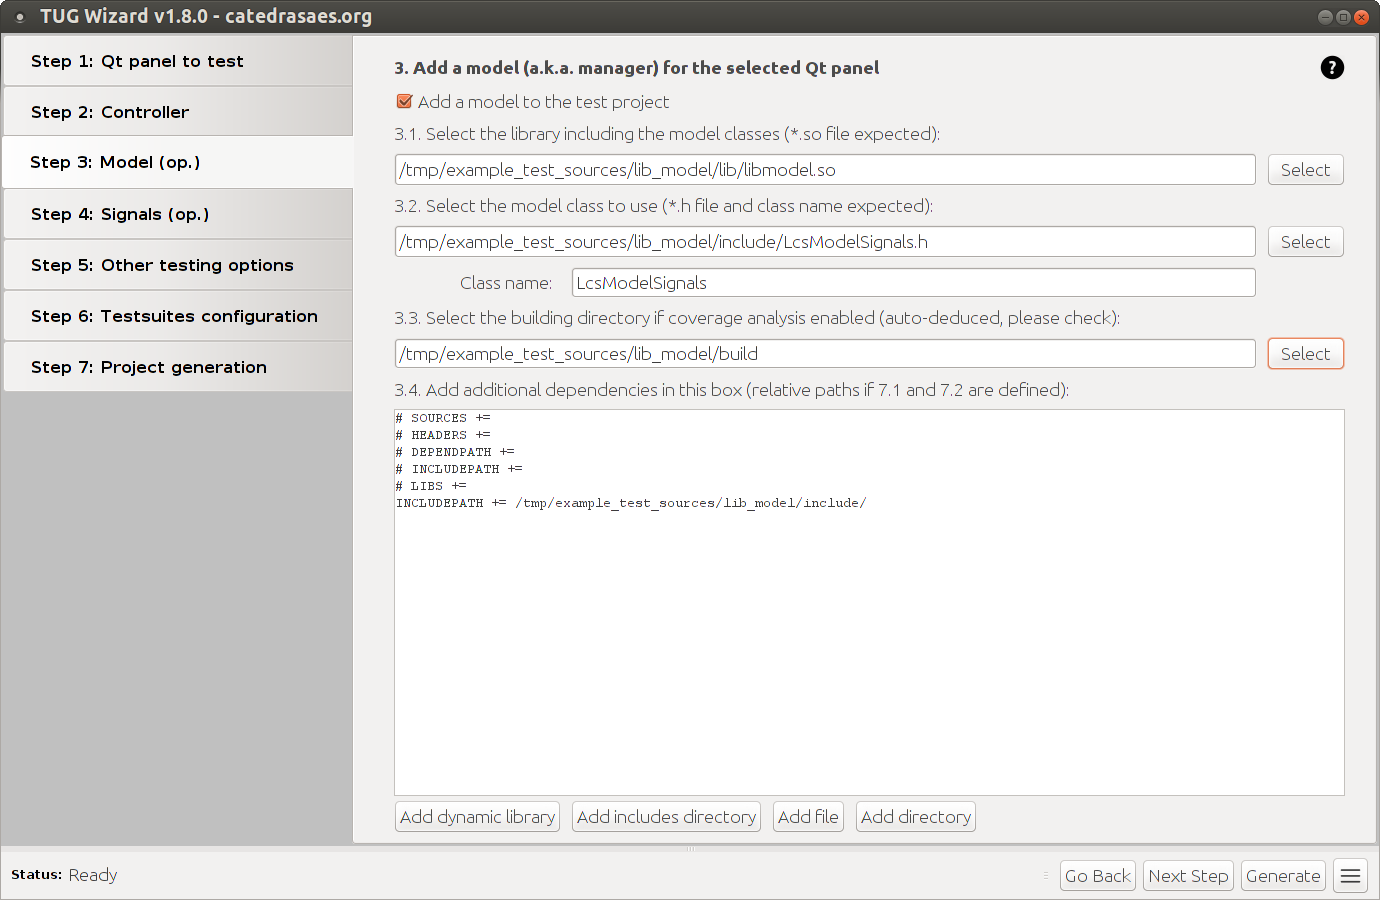
\includegraphics[width=.95\textwidth]{images/tug023.png}
\vspace{3ex}
\newpage
%
%%% 
%%
\item {\bf Step 4: Select a Signals class (optional).}\\
%
  You can select a class including those signals (S) used for the
  communication between GW and M.\\
%
  Check \field{Include a signals class into the testsuites} to enable this
  option.\\
%
  Click \field{4.1 Select} to choose the library containing the S class.\\
%
  Click \field{4.2 Select} to select the file defining the S
  class. \field{Class name} will be auto-filled based on the class name
  found in the selected file. Please, check it. \\
% 
  Click \field{4.3 Select} to select the directory in which S library is
  built. It is needed if coverage analysis is enabled.\\
%
  In \field{4.4} you can select if the signals used are based on {\tt
    Boost} or on {\tt Libsig}. You can select {\tt None} to add it
  manually. \field{Check/edit config file} can be used to check and edit
  the dependencies to be incorporated into the test project. \field{Back to
    default config} can be used to go back to default configuration of such
  dependencies. \\
%
  In \field{4.5} you can add additional dependencies for the S library.\\
%
  Click \field{Next Step} at the bottom of the wizard.

\vspace{3ex}
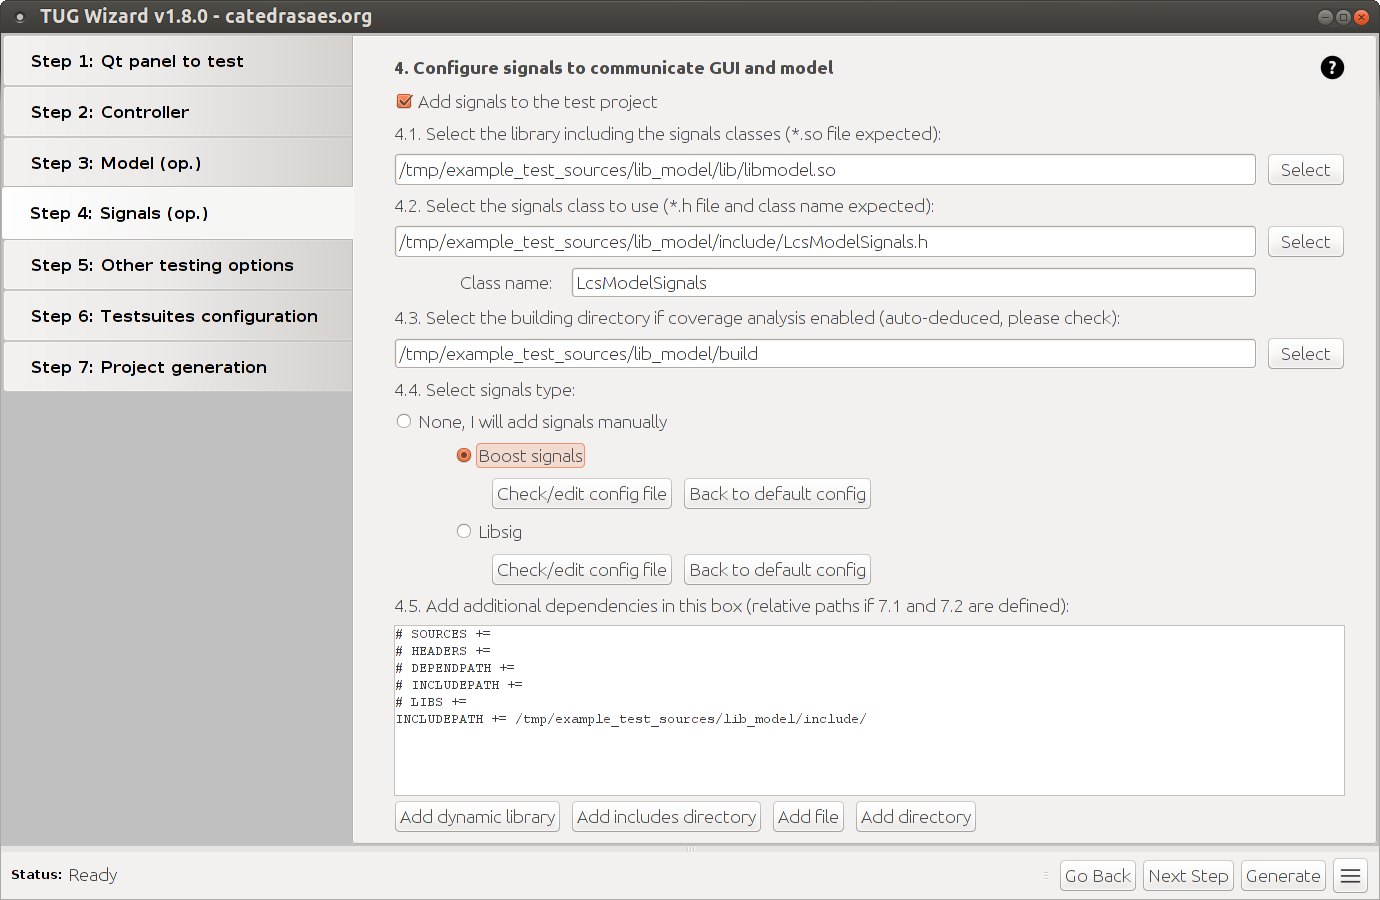
\includegraphics[width=.95\textwidth]{images/tug024.png}
\vspace{3ex}
\newpage
%
%%% 
%%
\item {\bf Step 5: Select other options for the test project.}\\
%
  In this step we can choose and configure options like coverage and
  profiling analysis, as well as add additional dependencies to the
  project.  In this step we can also check the includes for {\bf TUGLib},
  the library running under test projects generated by TUG Wizard.  \\
%
  Check \field{GCov enabled} to enable coverage analysis. \\
%
  Check \field{GProf enabled} to enable profiling. \\
%
  Check \field{Qwt enabled} to enable support for Qwt widgets. \\
%
  \field{Check/edit config file} can be used to check and edit the
  dependencies to be incorporated into the test project for each
  option. \field{Back to default config} can be used to go back to default
  configuration of such dependencies. \\
%
  In \field{5.4} you can add additional dependencies to the project. \\
%
  In \field{5.5} you can check, edit, and restore dependencies related to
  {\bf TUGLib} library.\\
%
  Click \field{Next Step} at the bottom of the wizard.

\vspace{3ex}
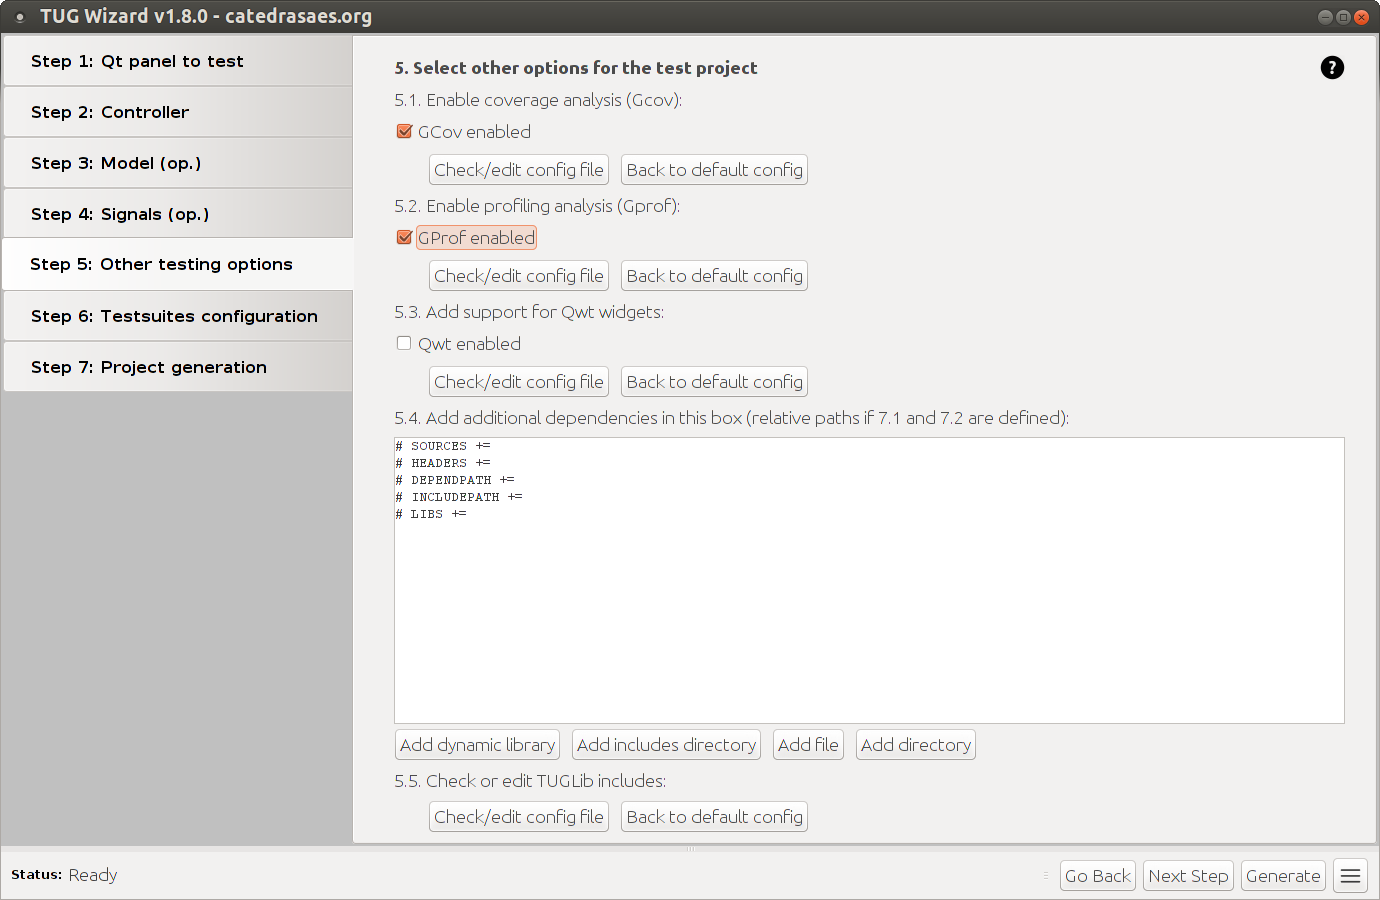
\includegraphics[width=.95\textwidth]{images/tug025.png}
\vspace{3ex}
\newpage
%
%%% 
%%
\item {\bf Step 6: Configure a testsuites structure (recommended).}\\
%
  In this step we can create the structure of a test project. As a result
  after the generation process, a set of testsuites will be auto-generated
  according to the test project configured in this step.\\
%
  Check \field{Generate test suites} to enable this option.  A
  pre-configured test project is provided as starting point. A test project
  is composed of a base testsuite (often used to configure and clean the
  test scenario) and a set of child testsuites that include some extra
  configuration (if needed) and the tests to be executed.  We can modify
  this test project as follows.\\
%
  Click \field{Add Test} to add a new test to a testsuite. Please,
  note that every testsuite (except base testsuite) must include, at
  least, one test.\\
%
  Click \field{Add Testsuite} to add a new child testsuite to a parent
  testsuite. Please, note that only level-2 testsuites are allowed
  (level-0 is base testsuite).\\
%
  Click \field{Delete Item} to delete selected item (either a test or
  a testsuite).\\
%
  Once the test project is created, click \field{Next Step} at the
  bottom of the wizard.\\
%
  \textcolor{red}{TUG Wizard implements {\bf roundtrip} between different
    versions of a test project. If a project is generated in the same
    directory it was generated before, then the code of old tests will
    be kept in the new version if they still exist.}

\vspace{3ex}
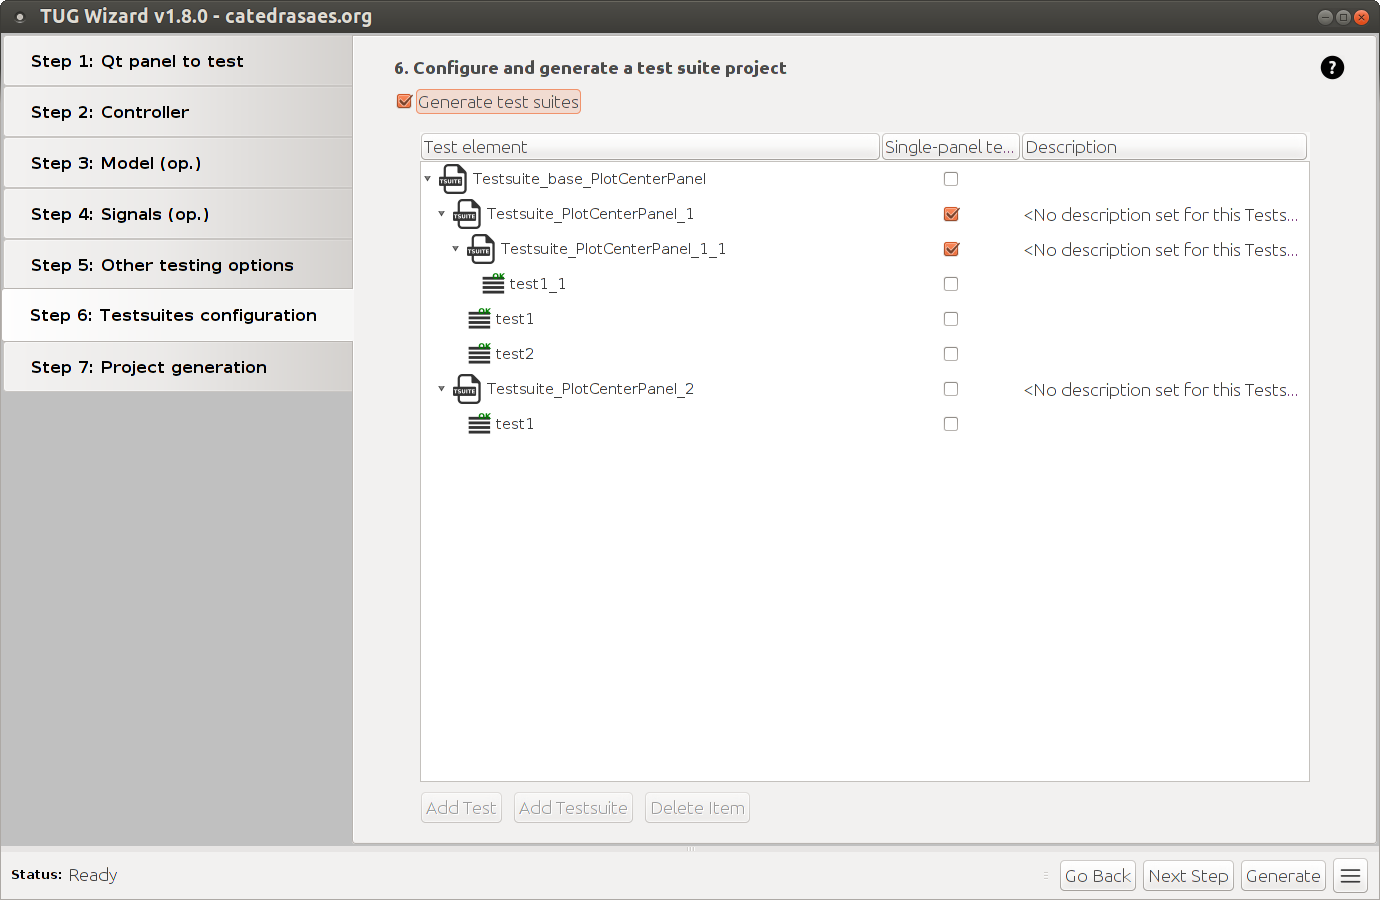
\includegraphics[width=.95\textwidth]{images/tug026.png}
\vspace{3ex}
\newpage
%
%%% 
%%
\item {\bf Step 7: Name the project and select a destination.}\\
%
  In \field{7.1} we have to add a name for our project. This name will be
  used to create a folder into which generate the project. It will be also
  used to identify the project within the output report.\\
%
  Click \field{7.2 Select} to select a directory into which generate the
  test project. Once selected, the label below this field will show the
  final destination of the test project.\\
%
  Click \field{Generate} at the bottom of the wizard to start the
  generation process. A console will appear showing generation process and
  result.

\vspace{3ex}
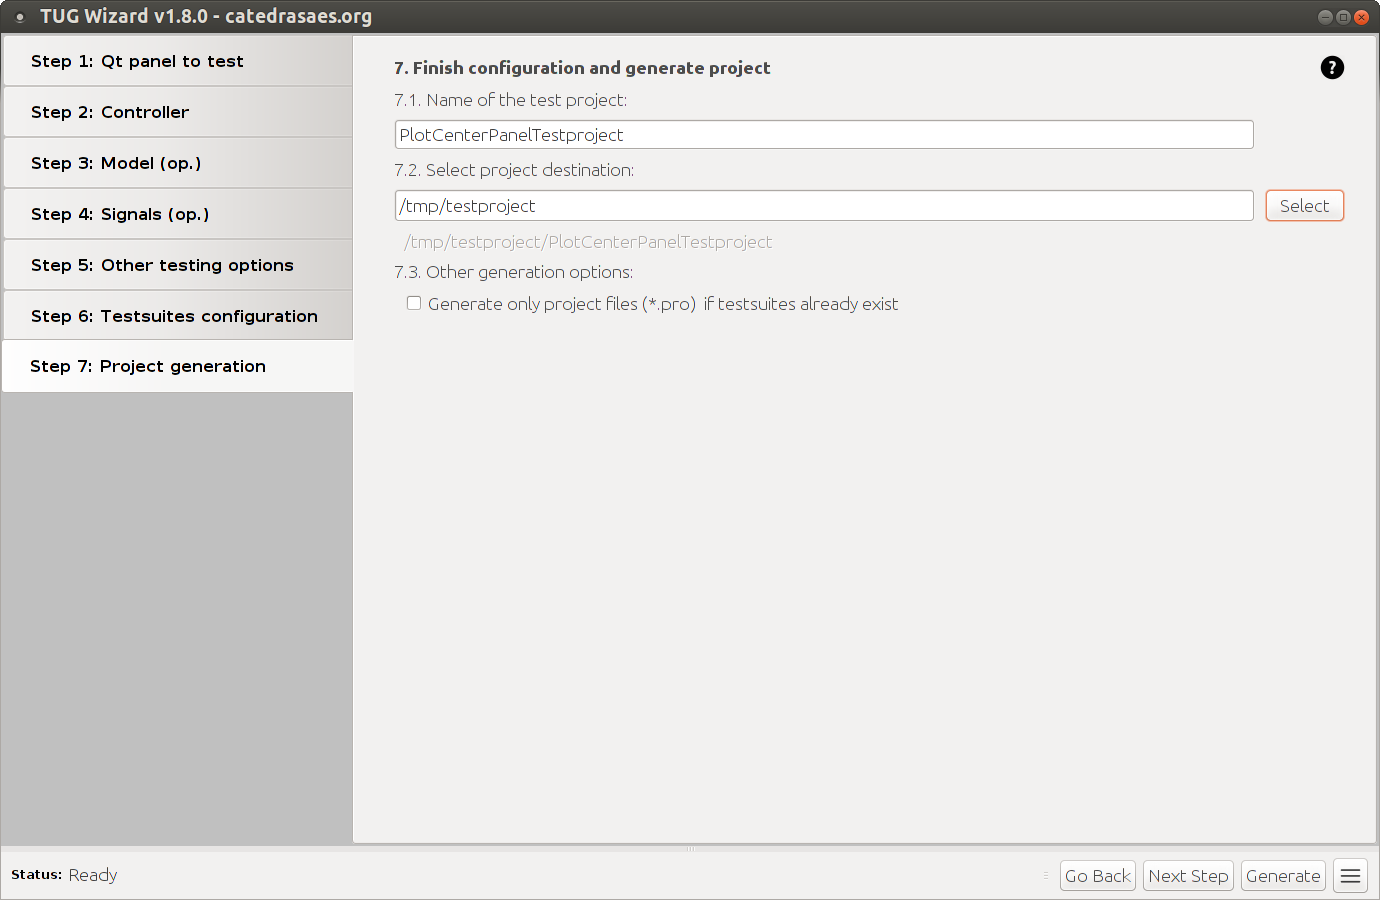
\includegraphics[width=.95\textwidth]{images/tug027.png}
\vspace{3ex}
%\newpage

%
%%% 
%%
\item {\bf Step 8: Exit the wizard.}\\
%
  Click 
\includegraphics[width=.05\textwidth]{images/menu_icon.png}
  to deploy the pop-up menu and select \field{Exit}.\\

\vspace{1ex}
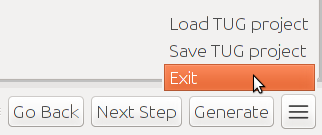
\includegraphics[width=.5\textwidth]{images/tug_exit.png}
\vspace{3ex}
\end{enumerate}
\newpage



%%% Local variables:
%%% mode: latex
%%% TeX-master: "README.tex"
%%% ispell-local-dictionary: "american"
%%% coding: utf-8
%%% fill-column: 75
%%% TeX-parse-self: t
%%% TeX-auto-save: t
%%% End:

